\documentclass[11pt,a4paper]{report}
\usepackage[textwidth=37em,vmargin=30mm]{geometry}
\usepackage{calc,xunicode,amsmath,amssymb,paralist,enumitem,tabu,booktabs,datetime2,xeCJK,xeCJKfntef,listings}
\usepackage{tocloft,fancyhdr,tcolorbox,xcolor,graphicx,eso-pic,xltxtra,xelatexemoji}

\newcommand{\envyear}[0]{2025}
\newcommand{\envdatestr}[0]{2025-08-02}
\newcommand{\envfinaldir}[0]{webdb/2025/20250802/final}

\usepackage[hidelinks]{hyperref}
\hypersetup{
    colorlinks=false,
    pdfpagemode=FullScreen,
    pdftitle={Web Digest - \envdatestr}
}

\setlength{\cftbeforechapskip}{10pt}
\renewcommand{\cftchapfont}{\rmfamily\bfseries\large\raggedright}
\setlength{\cftbeforesecskip}{2pt}
\renewcommand{\cftsecfont}{\sffamily\small\raggedright}

\setdefaultleftmargin{2em}{2em}{1em}{1em}{1em}{1em}

\usepackage{xeCJK,xeCJKfntef}
\xeCJKsetup{PunctStyle=plain,RubberPunctSkip=false,CJKglue=\strut\hskip 0pt plus 0.1em minus 0.05em,CJKecglue=\strut\hskip 0.22em plus 0.2em}
\XeTeXlinebreaklocale "zh"
\XeTeXlinebreakskip = 0pt


\setmainfont{Brygada 1918}
\setromanfont{Brygada 1918}
\setsansfont{IBM Plex Sans}
\setmonofont{JetBrains Mono NL}
\setCJKmainfont{Noto Serif CJK SC}
\setCJKromanfont{Noto Serif CJK SC}
\setCJKsansfont{Noto Sans CJK SC}
\setCJKmonofont{Noto Sans CJK SC}

\setlength{\parindent}{0pt}
\setlength{\parskip}{8pt}
\linespread{1.15}

\lstset{
	basicstyle=\ttfamily\footnotesize,
	numbersep=5pt,
	backgroundcolor=\color{black!5},
	showspaces=false,
	showstringspaces=false,
	showtabs=false,
	tabsize=2,
	captionpos=b,
	breaklines=true,
	breakatwhitespace=true,
	breakautoindent=true,
	linewidth=\textwidth
}






\newcommand{\coverpic}[2]{
    % argv: itemurl, authorname
    Cover photo by #2~~(\href{#1}{#1})
}
\newcommand{\makeheader}[0]{
    \begin{titlepage}
        % \newgeometry{hmargin=15mm,tmargin=21mm,bmargin=12mm}
        \begin{center}
            
            \rmfamily\scshape
            \fontspec{BaskervilleF}
            \fontspec{Old Standard}
            \fontsize{59pt}{70pt}\selectfont
            WEB\hfill DIGEST
            
            \vfill
            % \vskip 30pt
            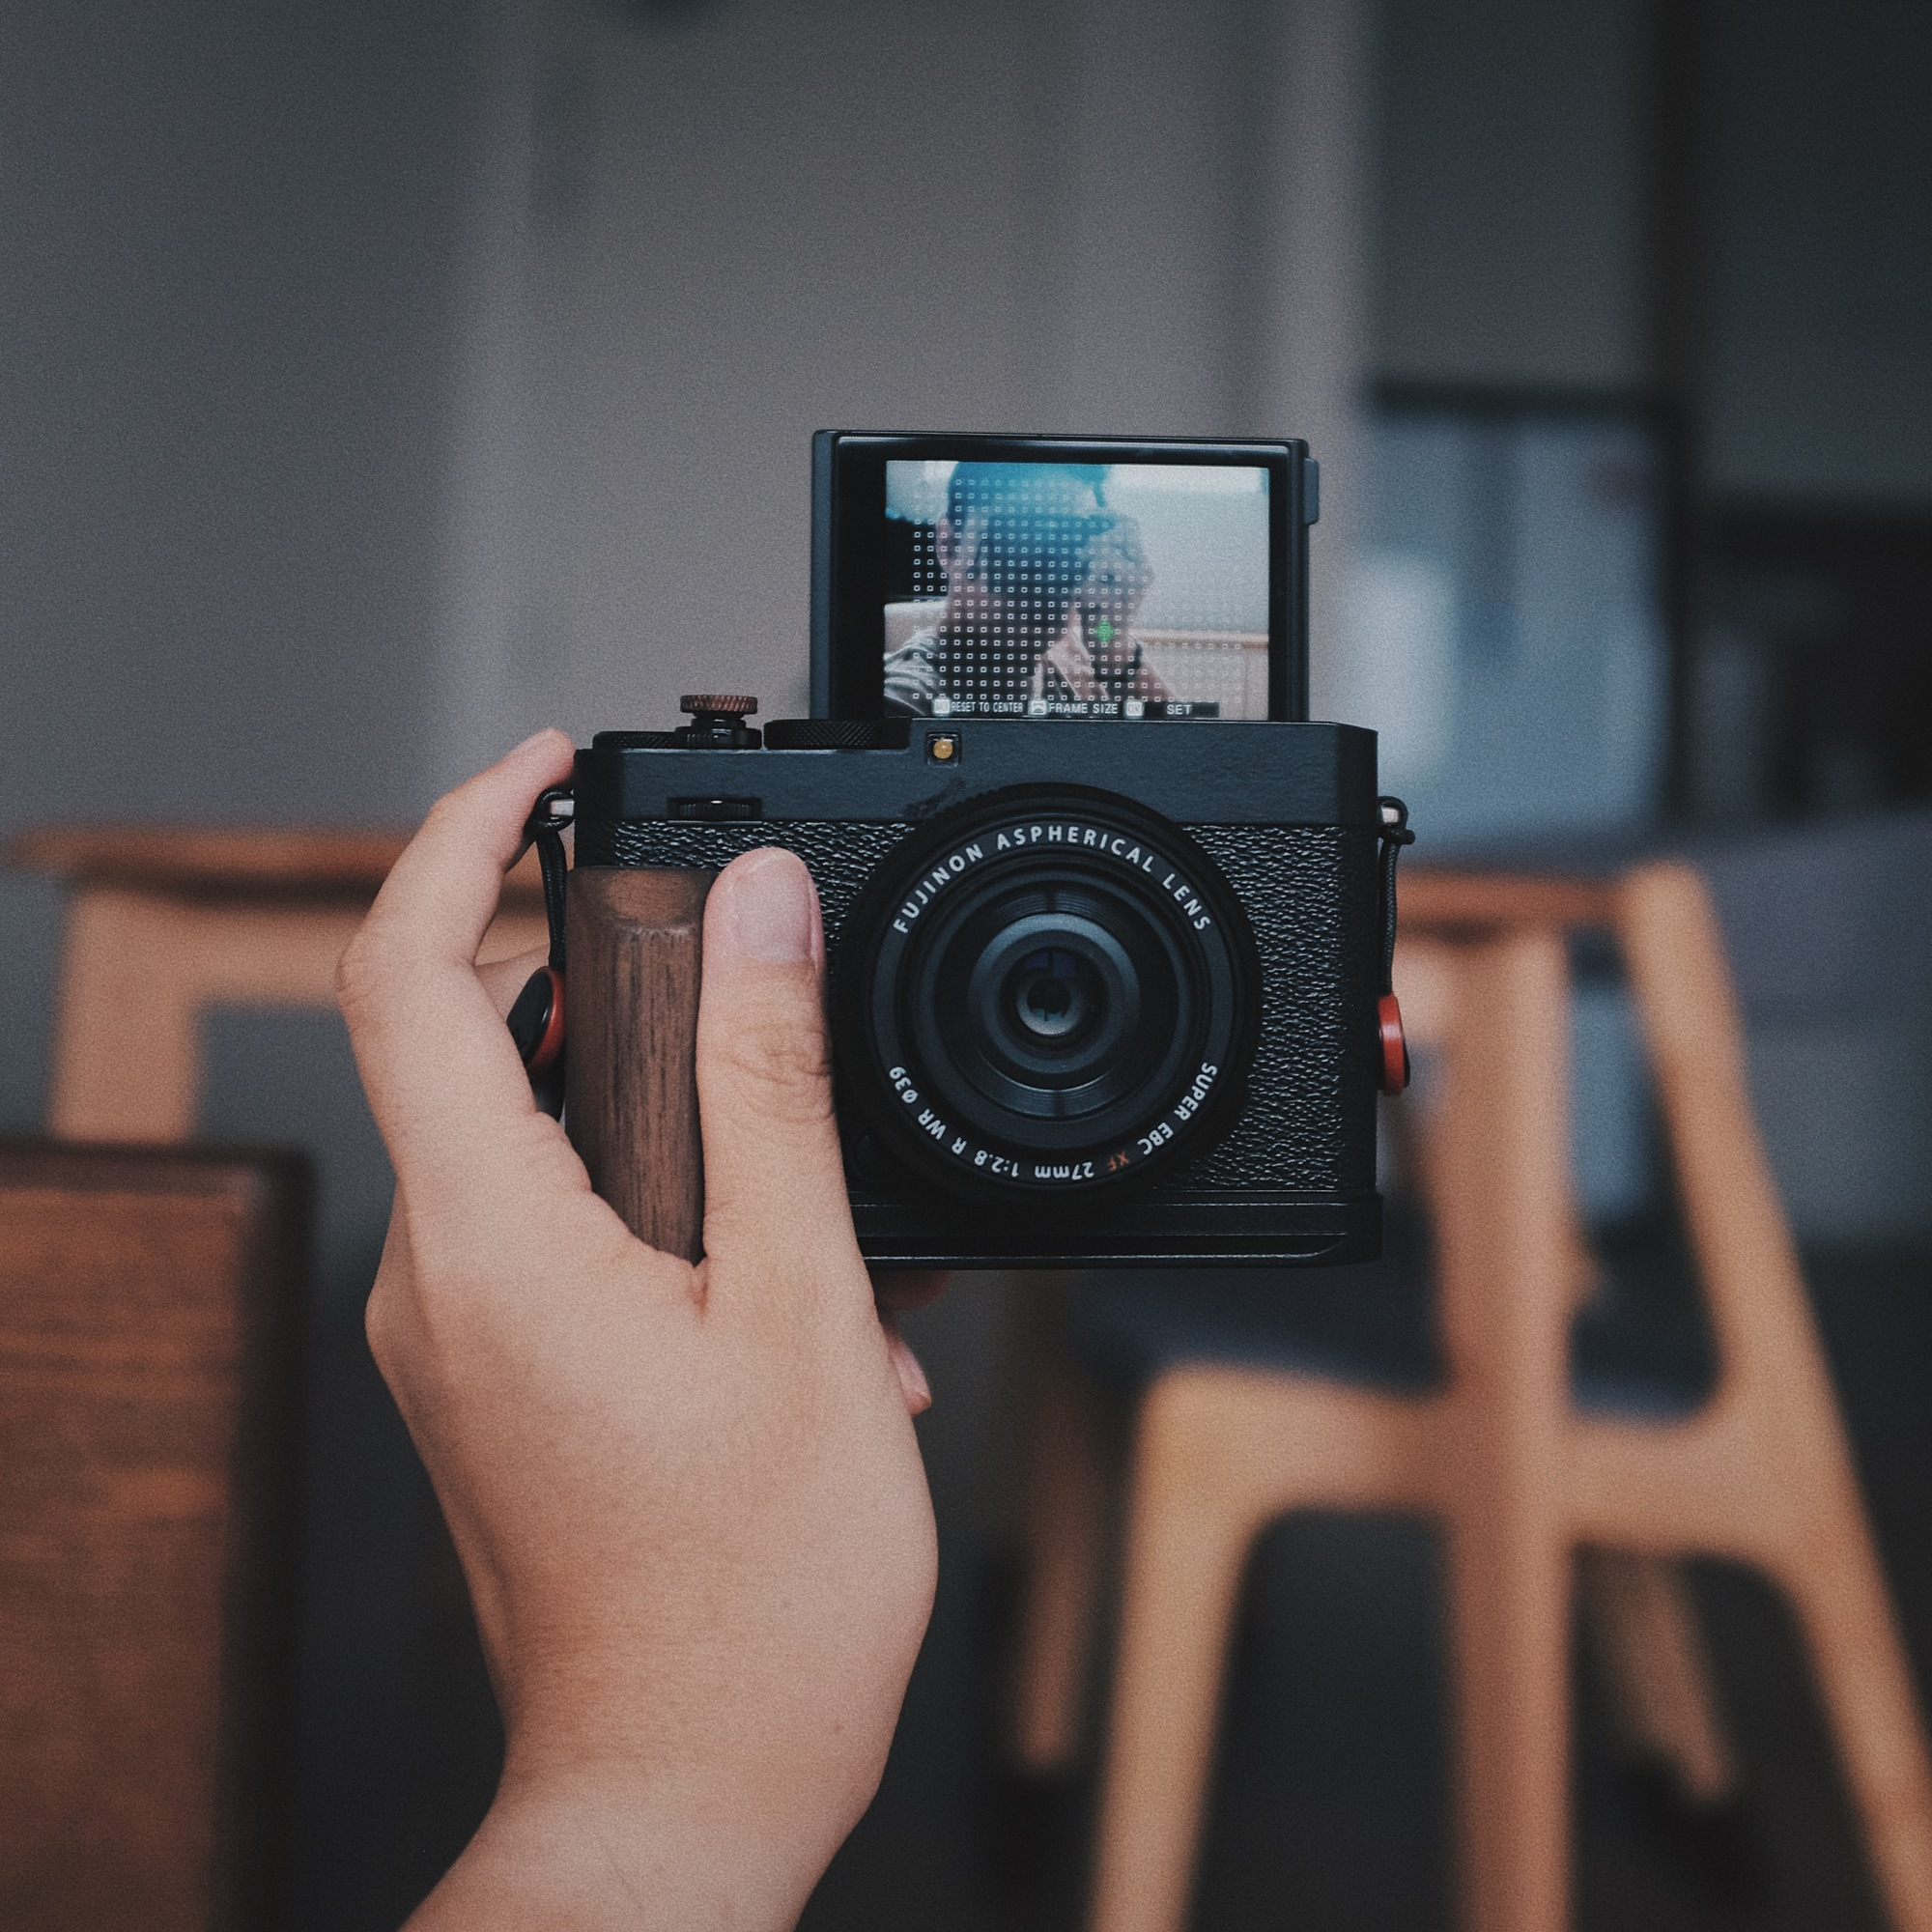
\includegraphics[width=\linewidth]{\envfinaldir/coverpic-prod.jpg}\par
            % \vskip 30pt
            \vfill

            \normalsize\rmfamily\scshape
            \copyright{} The Web Digest Project \hfill\large \envdatestr
        \end{center}
    \end{titlepage}
    % \restoregeometry
}
\newcommand{\simplehref}[1]{%
    \textcolor{blue!80!green}{\href{#1}{#1}}%
}
\renewcommand{\contentsname}{\center\Huge\sffamily\bfseries Contents\par\vskip 20pt}
\newcounter{ipartcounter}
\setcounter{ipartcounter}{0}
\newcommand{\ipart}[1]{
    % \vskip 20pt
    \clearpage
    \stepcounter{ipartcounter}
    \phantomsection
    \addcontentsline{toc}{chapter}{#1}
    % \begin{center}
    %     \Huge
    %     \sffamily\bfseries
    %     #1
    % \end{center}
    % \vskip 20pt plus 7pt
}
\newcounter{ichaptercounter}
\setcounter{ichaptercounter}{0}
\newcommand{\ichapter}[1]{
    % \vskip 20pt
    \clearpage
    \stepcounter{ichaptercounter}
    \phantomsection
    \addcontentsline{toc}{section}{\numberline{\arabic{ichaptercounter}}#1}
    \begin{center}
        \Huge
        \sffamily\bfseries
        #1
    \end{center}
    \vskip 20pt plus 7pt
}
\newcommand{\entrytitlefont}[1]{\subsection*{\raggedright\Large\sffamily\bfseries#1}}
\newcommand{\entryitemGeneric}[2]{
    % argv: title, url
    \parbox{\linewidth}{
        \entrytitlefont{#1}\par\vskip 5pt
        \footnotesize\ttfamily\mdseries
        \simplehref{#2}
    }\vskip 11pt plus 11pt minus 1pt
}
\newcommand{\entryitemGithub}[3]{
    % argv: title, url, desc
    \parbox{\linewidth}{
        \entrytitlefont{#1}\par\vskip 5pt
        \footnotesize\ttfamily\mdseries
        \simplehref{#2}\par\vskip 5pt
        \small\rmfamily\mdseries#3
    }\vskip 11pt plus 11pt minus 1pt
}
\newcommand{\entryitemAp}[3]{
    % argv: title, url, desc
    \parbox{\linewidth}{
        \entrytitlefont{#1}\par\vskip 5pt
        \footnotesize\ttfamily\mdseries
        \simplehref{#2}\par\vskip 5pt
        \small\rmfamily\mdseries#3
    }\vskip 11pt plus 11pt minus 1pt
}
\newcommand{\entryitemHackernews}[3]{
    % argv: title, hnurl, rawurl
    % \parbox{\linewidth}{
    %     \entrytitlefont{#1}\par\vskip 5pt
    %     \footnotesize\ttfamily\mdseries
    %     \simplehref{#3}\par
    %     \textcolor{black!50}{\href{#2}{#2}}
    % }\vskip 11pt plus 11pt minus 1pt
    \begin{minipage}{\linewidth}
            \entrytitlefont{#1}\par\vskip 5pt
            \footnotesize\ttfamily\mdseries
            \simplehref{#3}\par
            \textcolor{black!50}{\href{#2}{#2}}
    \end{minipage}\par\vskip 11pt plus 11pt minus 1pt
}







\begin{document}

\makeheader

\tableofcontents\clearpage




\ipart{Developers}
\ichapter{Hacker News}
\entryitemTwoLinks{Cerebras Code}{https://news.ycombinator.com/item?id=44762959}{https://www.cerebras.ai/blog/introducing-cerebras-code}

\entryitemTwoLinks{Atlassian terminates 150 staff}{https://news.ycombinator.com/item?id=44761205}{https://www.cyberdaily.au/digital-transformation/12441-atlassian-terminates-150-staff-with-pre-recorded-video-will-be-largely-replaced-by-ai}

\entryitemTwoLinks{Tesla must pay portion of \$329M damages after fatal Autopilot crash, jury says}{https://news.ycombinator.com/item?id=44760573}{https://www.cnbc.com/2025/08/01/tesla-must-pay-329-million-in-damages-in-fatal-autopilot-case.html}

\entryitemTwoLinks{Google shifts goo.gl policy: Inactive links deactivated, active links preserved}{https://news.ycombinator.com/item?id=44759918}{https://blog.google/technology/developers/googl-link-shortening-update/}

\entryitemTwoLinks{I couldn't submit a PR, so I got hired and fixed it myself}{https://news.ycombinator.com/item?id=44759417}{https://www.skeptrune.com/posts/doing-the-little-things/}

\entryitemTwoLinks{Corporation for Public Broadcasting ceasing operations}{https://news.ycombinator.com/item?id=44759382}{https://cpb.org/pressroom/Corporation-Public-Broadcasting-Addresses-Operations-Following-Loss-Federal-Funding}

\entryitemTwoLinks{At 17, Hannah Cairo solved a major math mystery}{https://news.ycombinator.com/item?id=44759152}{https://www.quantamagazine.org/at-17-hannah-cairo-solved-a-major-math-mystery-20250801/}

\entryitemTwoLinks{OpenAI Leaks 120B Open Model on Hugging Face}{https://news.ycombinator.com/item?id=44758511}{https://twitter.com/main\_horse/status/1951201925778776530}

\entryitemTwoLinks{FBI seized \$40k from Linda Martin without charging her with a crime}{https://news.ycombinator.com/item?id=44758339}{https://reason.com/2025/07/28/the-fbi-took-her-40000-without-explaining-why-she-fought-back-and-lost/}

\entryitemTwoLinks{Ask HN: Who is hiring? (August 2025)}{https://news.ycombinator.com/item?id=44757794}{https://news.ycombinator.com/item?id=44757794}

\entryitemTwoLinks{Long Term Support}{https://news.ycombinator.com/item?id=44757316}{https://www.sqlite.org/lts.html}

\entryitemTwoLinks{IRS head says free Direct File tax service is 'gone'}{https://news.ycombinator.com/item?id=44757262}{https://www.theverge.com/news/717308/irs-direct-file-gone-billy-long-trump-administration}

\entryitemTwoLinks{OpenAI raises \$8.3B at \$300B valuation}{https://news.ycombinator.com/item?id=44757247}{https://www.nytimes.com/2025/08/01/business/dealbook/openai-ai-mega-funding-deal.html}

\entryitemTwoLinks{GPT-5 is already (ostensibly) available via API}{https://news.ycombinator.com/item?id=44756314}{https://old.reddit.com/r/OpenAI/comments/1mettre/gpt5\_is\_already\_ostensibly\_available\_via\_api/}

\entryitemTwoLinks{Live coding interviews measure stress, not coding skills}{https://news.ycombinator.com/item?id=44756045}{https://hadid.dev/posts/living-coding/}

\entryitemTwoLinks{The untold impact of cancellation}{https://news.ycombinator.com/item?id=44755644}{https://pretty.direct/impact}

\entryitemTwoLinks{How did Facebook intercept competitor's encrypted mobile app traffic? (2024)}{https://news.ycombinator.com/item?id=44755528}{https://haxrob.net/onavo-facebook-ssl-mitm-technical-analysis/}

\entryitemTwoLinks{Belgium bans Internet Archive's `Open Library'}{https://news.ycombinator.com/item?id=44755441}{https://torrentfreak.com/belgium-bans-internet-archives-open-library-in-sweeping-site-blocking-order/}

\entryitemTwoLinks{NSF has suspended Terry Tao's grant}{https://news.ycombinator.com/item?id=44755429}{https://bsky.app/profile/dangaristo.bsky.social/post/3lvc7ldavhk2o}

\entryitemTwoLinks{Gemini 2.5 Deep Think}{https://news.ycombinator.com/item?id=44755279}{https://blog.google/products/gemini/gemini-2-5-deep-think/}


\ipart{Developers~~~~(zh-Hans)}
\ichapter{Solidot}
\entryitemGeneric{\hskip 0pt{}Google 将利用 AI 估算美国用户年龄}{https://www.solidot.org/story?sid=81945}

\entryitemGeneric{\hskip 0pt{}苹果二季度在华销售收入 153.7 亿美元}{https://www.solidot.org/story?sid=81944}

\entryitemGeneric{\hskip 0pt{}《战地6》的社区关卡编辑器使用开源引擎 Godot}{https://www.solidot.org/story?sid=81943}

\entryitemGeneric{\hskip 0pt{}为遏制登革热疫情巴西释放实验室培育的蚊子}{https://www.solidot.org/story?sid=81942}

\entryitemGeneric{\hskip 0pt{}英伟达宣布了结束旧架构 GPU 驱动支持的时间表}{https://www.solidot.org/story?sid=81941}

\entryitemGeneric{\hskip 0pt{}睡眠呼吸暂停口服药物即将面世}{https://www.solidot.org/story?sid=81940}

\entryitemGeneric{\hskip 0pt{}高铁的环境影响}{https://www.solidot.org/story?sid=81939}

\entryitemGeneric{\hskip 0pt{}人类每天在室内环境吸入逾 7 万个微塑料}{https://www.solidot.org/story?sid=81938}

\entryitemGeneric{\hskip 0pt{}人工甜味剂显著增加罹患糖尿病风险}{https://www.solidot.org/story?sid=81937}

\entryitemGeneric{\hskip 0pt{}研究显示限制 Google 付费成为默认搜索引擎能降低其市场份额}{https://www.solidot.org/story?sid=81936}

\entryitemGeneric{\hskip 0pt{}网信办约谈英伟达}{https://www.solidot.org/story?sid=81935}

\entryitemGeneric{\hskip 0pt{}AI 生成的代码近半包含安全漏洞}{https://www.solidot.org/story?sid=81934}

\entryitemGeneric{\hskip 0pt{}Vivo 宣布了用 Rust 开发的 BlueOS}{https://www.solidot.org/story?sid=81933}

\entryitemGeneric{\hskip 0pt{}澳大利亚儿童社媒禁令扩大到 YouTube}{https://www.solidot.org/story?sid=81932}

\entryitemGeneric{\hskip 0pt{}地球各大洲都经历淡水流失}{https://www.solidot.org/story?sid=81931}

\entryitemGeneric{\hskip 0pt{}愤怒的玩家对 Visa 和 Mastercard 的客服发动 DDoS 攻击}{https://www.solidot.org/story?sid=81930}

\entryitemGeneric{\hskip 0pt{}猫会让 AI 困惑}{https://www.solidot.org/story?sid=81929}

\entryitemGeneric{\hskip 0pt{}Google 鼓励员工使用 AI}{https://www.solidot.org/story?sid=81928}

\entryitemGeneric{\hskip 0pt{}Futurehome 申请破产后推送固件移除设备本地功能强推订阅制}{https://www.solidot.org/story?sid=81927}

\entryitemGeneric{\hskip 0pt{}微软承认它无法保障欧洲国家的数字主权}{https://www.solidot.org/story?sid=81926}\ichapter{V2EX}
\entryitemGeneric{\hskip 0pt{}[服务器] gpu 服務器還有哪裏更便宜?}{https://www.v2ex.com/t/1149411}

\entryitemGeneric{\hskip 0pt{}[Go 编程语言] bufbuild/protovalidate 如何判断 string 是否为空跟未设置}{https://www.v2ex.com/t/1149410}

\entryitemGeneric{\hskip 0pt{}[程序员] 谈到工作之外的技术热情,我也请教一个问题}{https://www.v2ex.com/t/1149409}

\entryitemGeneric{\hskip 0pt{}[Apple] iOS26 系统 image picker 史诗级增强?}{https://www.v2ex.com/t/1149408}

\entryitemGeneric{\hskip 0pt{}[宽带症候群] 询问中兴光猫 需求口子开 hybird 模式}{https://www.v2ex.com/t/1149406}

\entryitemGeneric{\hskip 0pt{}[问与答] 有没有什么支持在 ssh 输出端处理数据的 ssh 客户端?}{https://www.v2ex.com/t/1149405}

\entryitemGeneric{\hskip 0pt{}[VXNA] VXNA 聚合了很多 RSS,而它本身也是一个 RSS,不用一直刷页面,订阅就好了}{https://www.v2ex.com/t/1149404}

\entryitemGeneric{\hskip 0pt{}[汽车] 深度体验特斯拉感受}{https://www.v2ex.com/t/1149403}

\entryitemGeneric{\hskip 0pt{}[美国] NYT Connections Answers \& Hints}{https://www.v2ex.com/t/1149402}

\entryitemGeneric{\hskip 0pt{}[iPhone] 之前有大佬推荐一个管理订阅的 app 大佬有知道是什么么?}{https://www.v2ex.com/t/1149401}

\entryitemGeneric{\hskip 0pt{}[职场话题] 有 Java 后端社招的一起线上共享信息,一起找工作吗?}{https://www.v2ex.com/t/1149400}

\entryitemGeneric{\hskip 0pt{}[问与答] 有好心人能帮忙发个帖吗- -}{https://www.v2ex.com/t/1149399}

\entryitemGeneric{\hskip 0pt{}[宽带症候群] 直接连接 RustDesk 显示连接被对方关闭,无法连接}{https://www.v2ex.com/t/1149398}

\entryitemGeneric{\hskip 0pt{}[iPhone] 问下:没备份的情况下,升级到 iOS 26,有办法保留数据的前提下回滚到 18.6 吗?}{https://www.v2ex.com/t/1149397}

\entryitemGeneric{\hskip 0pt{}[分享创造] 使用 gemini-CLI 五分钟解决了烦人的 HDR 头像问题}{https://www.v2ex.com/t/1149396}

\entryitemGeneric{\hskip 0pt{}[问与答] notion 的垃圾箱超过一个月,还有什么办法能找回来吗。}{https://www.v2ex.com/t/1149395}

\entryitemGeneric{\hskip 0pt{}[分享创造] 开源了一个让 Roo Code 可以运行在 Jetbrains 平台的 IDE 插件}{https://www.v2ex.com/t/1149394}

\entryitemGeneric{\hskip 0pt{}[分享创造] 我花 1 个月做了一个技术社区!}{https://www.v2ex.com/t/1149393}

\entryitemGeneric{\hskip 0pt{}[问与答] 有用过 gcore 他们家的 cdn 的朋友吗?感觉速度怎么样}{https://www.v2ex.com/t/1149392}

\entryitemGeneric{\hskip 0pt{}[程序员] 微信电话在 ios 端的那种持续震动加声音的通知(非 callkit)怎么实现的?}{https://www.v2ex.com/t/1149391}

\entryitemGeneric{\hskip 0pt{}[职场话题] 自由职业虽好,但是比上班更累.....你们真的会选择吗?}{https://www.v2ex.com/t/1149390}

\entryitemGeneric{\hskip 0pt{}[问与答] 显示器用了三年了,时不时亮度忽明忽暗,然后过一会就好了,是没救了吗}{https://www.v2ex.com/t/1149389}

\entryitemGeneric{\hskip 0pt{}[问与答] 各位大佬前辈们,求一个馒头 pt💊}{https://www.v2ex.com/t/1149385}

\entryitemGeneric{\hskip 0pt{}[微信] 微信作为一个全家桶超级应用 是否应该将聊天功能剥离}{https://www.v2ex.com/t/1149384}

\entryitemGeneric{\hskip 0pt{}[远程工作] 远程办公, SEO 开发工程师}{https://www.v2ex.com/t/1149383}

\entryitemGeneric{\hskip 0pt{}[Solana] 新用户注册 OKX 交易所赠送 500 枚\$V2EX}{https://www.v2ex.com/t/1149382}

\entryitemGeneric{\hskip 0pt{}[推广] 3 分钟注册 币安 即领 666 枚 \$V2EX}{https://www.v2ex.com/t/1149380}

\entryitemGeneric{\hskip 0pt{}[程序员] 前端转全栈, AI 时代搞个啥项目练手比较有亮点?}{https://www.v2ex.com/t/1149379}

\entryitemGeneric{\hskip 0pt{}[NAS] 极摩客 K12 看参数和介绍是一个我心目中的六边形战士}{https://www.v2ex.com/t/1149378}

\entryitemGeneric{\hskip 0pt{}[宽带症候群] 献给所有的留学生哈基米:琢磨了个能同时留学和回家的方案,不需要公网 ip}{https://www.v2ex.com/t/1149377}

\entryitemGeneric{\hskip 0pt{}[问与答] 很老的一个移动卡,动感地带, 2G 的卡,一直用来收短信,最近收不到}{https://www.v2ex.com/t/1149375}

\entryitemGeneric{\hskip 0pt{}[React] 谁有闲工夫, React,帮忙定位并处理下 BUG}{https://www.v2ex.com/t/1149374}

\entryitemGeneric{\hskip 0pt{}[问与答] 家里小孩整天看腾讯视频,有什么办法,在不碰他电脑的情况下,让他访问腾讯视频时跳到一个恶搞页面 😤😤}{https://www.v2ex.com/t/1149373}

\entryitemGeneric{\hskip 0pt{}[生活] 今天去看了心理医生,医生说是抑郁状态}{https://www.v2ex.com/t/1149372}

\entryitemGeneric{\hskip 0pt{}[iPad] 妙控键盘的触摸板是不是实用性不高?}{https://www.v2ex.com/t/1149370}

\entryitemGeneric{\hskip 0pt{}[分享创造] 注销么?列举手机号码可能注册过的平台}{https://www.v2ex.com/t/1149369}

\entryitemGeneric{\hskip 0pt{}[分享发现] Jetbrains 全系产品 2025 年 10 月 1 日起再次涨价}{https://www.v2ex.com/t/1149368}

\entryitemGeneric{\hskip 0pt{}[路由器] Wi-Fi 连接正常但是无法联网}{https://www.v2ex.com/t/1149367}

\entryitemGeneric{\hskip 0pt{}[macOS] MacOS FaceTime 回音的问题求助}{https://www.v2ex.com/t/1149366}

\entryitemGeneric{\hskip 0pt{}[远程工作] [远程办公/全球招募/Web3 钱包] 资深前/后端工程师/产品经理}{https://www.v2ex.com/t/1149365}

\entryitemGeneric{\hskip 0pt{}[分享发现] 推荐给后端小哥看本站 v 友的寻求方案链接 QWQ}{https://www.v2ex.com/t/1149361}

\entryitemGeneric{\hskip 0pt{}[VXNA] 申请收录个人博客: https://liujiale.me}{https://www.v2ex.com/t/1149360}

\entryitemGeneric{\hskip 0pt{}[问与答] 如何最低成本可以让自己每年都用上 iPhone 的新款手机呢?}{https://www.v2ex.com/t/1149359}

\entryitemGeneric{\hskip 0pt{}[问与答] 给别人建网站的收费}{https://www.v2ex.com/t/1149358}

\entryitemGeneric{\hskip 0pt{}[Apple] 闲鱼买的美版 Mac Studio 加入了 Apple One Care}{https://www.v2ex.com/t/1149357}

\entryitemGeneric{\hskip 0pt{}[Solana] 兑换 \$V2EX gas 不足}{https://www.v2ex.com/t/1149356}

\entryitemGeneric{\hskip 0pt{}[程序员] Next.js 中用什么来管理全局状态,类似 Vuex/Pinia ?}{https://www.v2ex.com/t/1149355}

\entryitemGeneric{\hskip 0pt{}[分享发现] 用 Claude Code 撸了一个 AI 视频生成网站}{https://www.v2ex.com/t/1149354}

\entryitemGeneric{\hskip 0pt{}[分享创造] 为了方便自己互联网冲浪品到细糠做记录又搞了一个落地页导航站}{https://www.v2ex.com/t/1149353}

\entryitemGeneric{\hskip 0pt{}[反馈] 为什么交易区发布帖子,直接到第二页了?}{https://www.v2ex.com/t/1149351}


\ipart{Generic News}







\clearpage
\leavevmode\vfill
\footnotesize

Copyright \copyright{} 2023-2025 Neruthes and other contributors.

This document is published with CC BY-NC-ND 4.0 license.

The entries listed in this newsletter may be copyrighted by their respective creators.

This newsletter is generated by the Web Digest project.

The newsletters are also delivered via Telegram channel \CJKunderline{\href{https://t.me/webdigestchannel}{https://t.me/webdigestchannel}}.\\
RSS feed is available at \CJKunderline{\href{https://webdigest.pages.dev/rss.xml}{https://webdigest.pages.dev/rss.xml}}.

This newsletter is available in PDF at
\CJKunderline{\href{https://webdigest.pages.dev/}{https://webdigest.pages.dev/}}.

The source code being used to generate this newsletter is available at\\
\CJKunderline{\href{https://github.com/neruthes/webdigest}{https://github.com/neruthes/webdigest}}.

This newsletter is also available in
\CJKunderline{\href{http://webdigest.pages.dev/readhtml/\envyear/WebDigest-20250802.html}{HTML}} and
\CJKunderline{\href{https://github.com/neruthes/webdigest/blob/master/markdown/\envyear/WebDigest-20250802.md}{Markdown}}.


\coverpic{https://unsplash.com/photos/a-tree-silhouetted-against-a-sunset-sky-AuVYd7aR5a4}{Peter Thomas}


\end{document}
